% Edit this section directly. Styling is in raylo-report.sty.
\section{Adding text to the risk model}
A separate programme, run in its own repository over the first week of September, asked a different question. The champion sees each applicant as a table of category counts. Could a model that reads the applicant's raw transaction sequence, in order, with the bank's own wording, find signal that the counts lose? This is the thesis behind several published ``transaction foundation model'' efforts, and it was tested here in two stages.

\subsection{How the two learned scores work}
Both approaches in this section end the same way: as a single number per applicant that is handed to the tree model as one more column. They differ in what they read.

\textbf{The text encoder} is the same kind of encoder transformer described in section 9, but used without any fine-tuning. An off-the-shelf model (bge-base, trained by its authors on general English) reads each bank narrative and produces a 768-number summary. Those summaries are averaged across all of an applicant's transactions, so the result is one vector describing the flavour of their statement as a whole, without any category having been assigned. A small logistic model, fitted on our own outcome data, turns that vector into one risk score. Nothing in this path knows about our taxonomy; it captures whatever the wording of the transactions says that the categories do not.

\textbf{The sequence transformer} reads the applicant, not the narrative. Each transaction becomes one event carrying its amount band, its timing relative to the application, its direction, the taxonomy leaf our categoriser gave it, and a compressed text vector. The events are laid out in date order, up to 1,024 of them, and a transformer reads the whole sequence at once, so a payday loan the day after a gambling spree can be understood as a pattern rather than two separate counts. It was pretrained on 48,000 applicants' histories with the sequence version of fill-in-the-blank, hiding one event and asking the model to reconstruct it, and then a small head was trained on repayment outcomes. Its output is again one number per applicant.

\begin{figure}[H]
\centering
\ChartTitle{Figure 8a. How the two learned scores are produced for one applicant}
\resizebox{\linewidth}{!}{%
\begin{tikzpicture}[
  x=1mm,y=1mm,font=\footnotesize,
  box/.style={draw=Blue,fill=BlueTint,rounded corners=1.2mm,line width=0.4pt,align=center,inner sep=2mm,text width=34mm},
  boxp/.style={draw=Peach,fill=PeachTint,rounded corners=1.2mm,line width=0.4pt,align=center,inner sep=2mm,text width=34mm},
  data/.style={draw=Muted,fill=white,rounded corners=1.2mm,line width=0.4pt,align=left,inner sep=2mm,text width=40mm},
  result/.style={draw=Blue,fill=Blue,text=white,rounded corners=1.2mm,line width=0.4pt,align=center,inner sep=2mm,text width=34mm},
  lab/.style={font=\scriptsize\color{Muted},align=left},
  arr/.style={-{Stealth[length=2mm]},line width=0.5pt,color=Muted}]
  \node[data,text width=44mm] (app) at (0,-8) {\textbf{One applicant, 90 days}\\about 300 transactions, each with date, amount, direction, narrative and our category};
  % text path
  \node[lab,anchor=west] at (54,22) {\textbf{Text score} (locked)};
  \node[box] (enc) at (74,8) {\textbf{Text encoder}\\bge-base reads each narrative\\$\rightarrow$ 300 vectors of 768 numbers};
  \node[box] (mean) at (118,8) {\textbf{Average}\\one vector for the whole statement};
  \node[result] (probe) at (162,8) {\textbf{Probe}\\logistic fit on outcomes\\$\rightarrow$ one score};
  % sequence path
  \node[lab,anchor=west] at (54,-14) {\textbf{Sequence-encoder score} (challenger)};
  \node[boxp] (ev) at (74,-28) {\textbf{Events in date order}\\amount band, timing, direction, taxonomy leaf, text vector};
  \node[boxp] (seq) at (118,-28) {\textbf{Sequence transformer}\\15M parameters, frozen; attends across all events};
  \node[result] (head) at (162,-28) {\textbf{Attention head}\\trained on outcomes\\$\rightarrow$ one score};
  % xgb
  \node[data,text width=40mm] (xgb) at (212,-10) {\textbf{Risk model}\\single XGBoost on 50 taxonomy features + text score (+ encoder score in the challenger recipe)\\$\rightarrow$ probability of default};
  \node[lab,anchor=north,align=center] (feat) at (212,-30) {the 50 taxonomy features come\\from the categorised transactions\\(section 10)};
  \draw[arr] (app.east) -- ++(4,0) |- (enc.west);
  \draw[arr] (app.east) -- ++(4,0) |- (ev.west);
  \draw[arr] (enc) -- (mean); \draw[arr] (mean) -- (probe);
  \draw[arr] (ev) -- (seq); \draw[arr] (seq) -- (head);
  \draw[arr] (probe.east) -- ++(3,0) |- ([yshift=4mm]xgb.west);
  \draw[arr,dashed] (head.east) -- ++(3,0) |- ([yshift=-4mm]xgb.west);
  \draw[arr] (feat.north) -- (xgb.south);
\end{tikzpicture}}
\caption*{Both paths reduce an applicant's transactions to one number that the tree model treats like any other feature. The text path runs one frozen encoder; the sequence path needs the categoriser's leaf, a second text encoder for its inputs, and the sequence model itself, which is why it is the challenger rather than the primary recipe.}
\end{figure}

What this means for the risk model: the trees already see how much, how often and in how many months each category appears. The text score adds what the words say beyond the category, for instance that an ``unclassified transfer'' narrative reads like a loan repayment. The sequence score adds order and timing, which counts lose. Neither replaces the trees; each supplies one column the trees could not compute for themselves, and the results below show how much each column is worth.

\subsection{Stage one: do text embeddings carry credit signal at all}
The cheapest test first. Each distinct bank narrative (2.9 million strings) was turned into a vector by a frozen off-the-shelf sentence encoder, the vectors were averaged per applicant, and a logistic regression was fitted on the average. With no categories and no hand-built features, that probe matched the production-spec GBM refit on the same population. The text does carry signal. Compressed to 32 columns and added to the taxonomy model, it gave a small and unstable lift.

\subsection{Stage two: a sequence transformer over transactions}
A transformer was then built to read up to 1,024 transactions per applicant, each represented by its amount bucket, timing, direction and text vector. It was pretrained with a masked-event objective, the sequence equivalent of fill-in-the-blank, on 48,000 applicants' histories, and read out first with a linear probe and later with fine-tuning. The versions are worth listing because each was built to test one thing.


{\small
\setlength{\TableWidth}{\dimexpr\linewidth-8\tabcolsep\relax}
\begin{longtable}{>{\raggedright\arraybackslash}p{0.16\TableWidth}>{\raggedright\arraybackslash}p{0.36\TableWidth}>{\raggedright\arraybackslash}p{0.33\TableWidth}>{\raggedright\arraybackslash}p{0.15\TableWidth}}
\rowcolor{BlueTint}
\bfseries Version & \bfseries What changed & \bfseries Why & \bfseries GINI, six-month \\ \midrule
\endfirsthead
\rowcolor{BlueTint}
\bfseries Version & \bfseries What changed & \bfseries Why & \bfseries GINI, six-month \\ \midrule
\endhead
v1 & 5 million parameters, raw fields only, 26 laptop-minutes & Establish a floor & 0.450 \\ \addlinespace[4pt]
v2, v3 & Longer training; 56\% more data including unlabelled recent applicants & Rule out data and training length as the limit & 0.473 \\ \addlinespace[4pt]
v4 & Each transaction also carries our taxonomy leaf as an input token & Test whether the model needs categories or can derive them & 0.546 \\ \addlinespace[4pt]
v5 & Leaf token made provider-blind (general category where the leaf came from a provider crosswalk) & The raw leaf let the model identify the provider perfectly, which would not transfer & 0.561 \\ \addlinespace[4pt]
v5 fine-tuned & Full fine-tuning with attention pooling & Test whether the readout, not the representation, was the limit & 0.551 \\ \addlinespace[4pt]
v6 & Three times the parameters (15 million) & Test capacity & 0.576 to 0.586 \\ \addlinespace[4pt]
\rowcolor{PeachTint}
Champion, refit on the same population &  &  & 0.616 \\ \addlinespace[4pt]
\bottomrule
\end{longtable}}
\begin{figure}[H]
\centering
\ChartTitle{Figure 9. Sequence transformer versions against the champion, six-month GINI on 6,252 applicants}
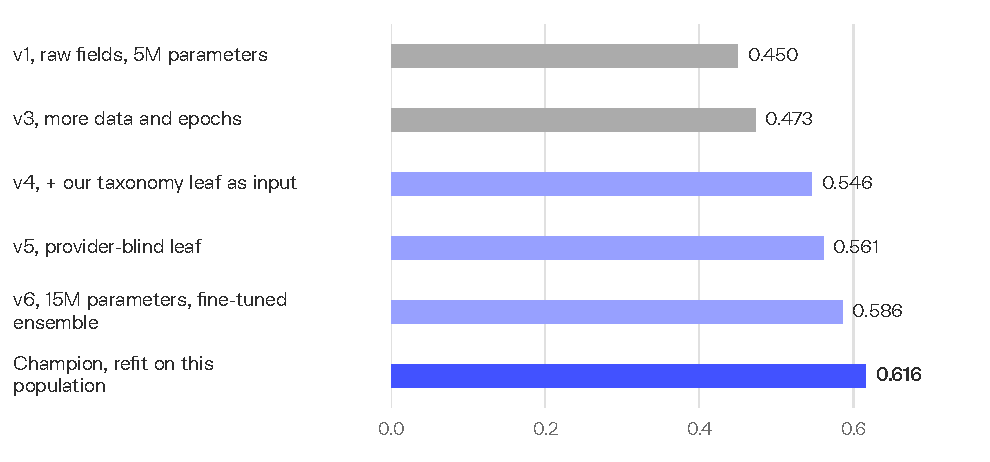
\includegraphics[width=\linewidth]{charts/fig-seq.pdf}
\caption*{The step from v3 to v4 is the category token. Everything after it is inside the noise of 397 bad outcomes. Stacked on the champion, no version added a significant gain.}
\end{figure}
The pattern is clear in hindsight. Without categories the sequence model plateaued at about 0.47 regardless of data or epochs. Given our leaf as an input, it jumped to the level of the 50-feature taxonomy XGBoost. Every further lever, fine-tuning, attention pooling and tripling the size, moved it a little, and the best configuration is statistically level with the champion but below it on both metrics. The bigger model overfitted within two epochs because there are only 2,200 bad outcomes to learn from; label scarcity, not model capacity, capped every configuration.

The sequence-model results in this section were measured against the uncapped champion, refit on that repository's population (GINI 0.616). The text-score stacking was then re-run against the 50-feature capped champion once it became the reference; those results are at the end of the section.

Stacked on the uncapped champion as an extra feature, the sequence model added nothing significant. The champion's thousands of leaf-level columns already contain what the sequence model had learned from categories, and at that point it was parked. The picture changed once the 50-feature capped champion became the reference, as the last part of this section shows.

\subsection{What did add value: one text score}
What remains in the raw text after the categories are accounted for is small but real, and the simplest extraction captures it. A frozen sentence encoder embeds each description, the vectors are averaged per applicant, and a small logistic model turns the average into one risk score, added to the champion as a single column. That single number beat 32 compressed columns, and it is far easier to monitor.

Eight encoders were compared in that role, from 22 million to 568 million parameters, including our own domain-pretrained DistilBERT from section 9. All landed in one narrow band of roughly +0.01 PR-AUC on the champion. Encoder size and family do not matter here, which is itself informative: the lift is a property of the residual free text, not of the encoder. bge-base was chosen because both of its deltas exclude zero and it runs on a laptop CPU. Our own encoder was fractionally ahead on the point estimate and half the cost to run, but not distinguishably better, and it had seen the test period's text during unsupervised pretraining, so it is recorded as the preferred replacement candidate pending the prospective test.

\begin{figure}[H]
\centering
\ChartTitle{Figure 10. PR-AUC lift from one text score, on the uncapped and the 50-feature champion (95\% CIs)}
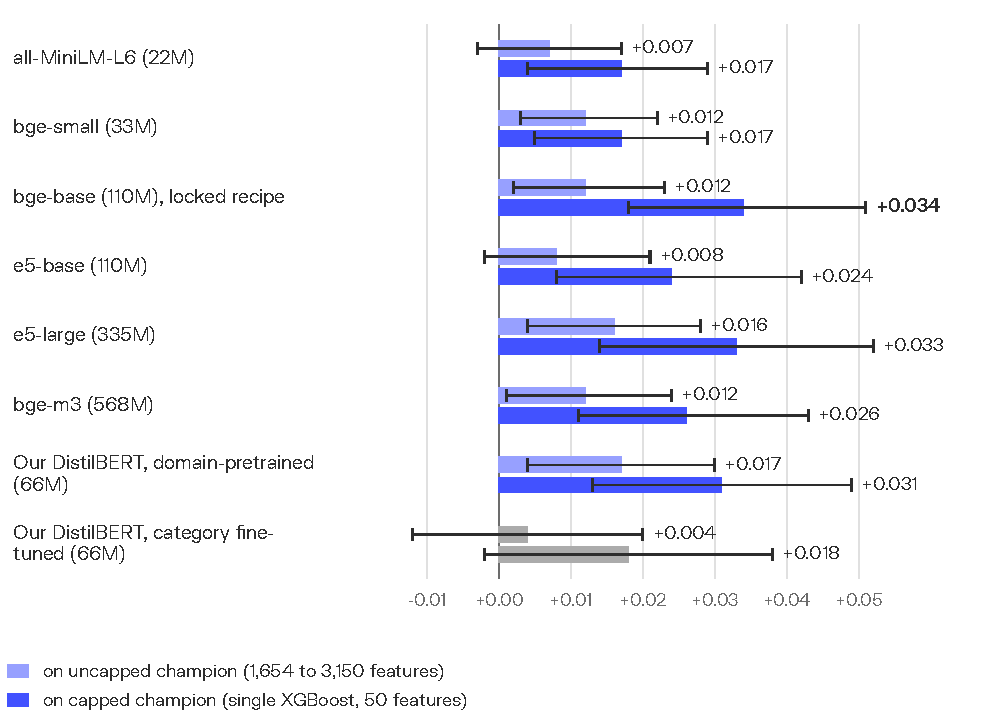
\includegraphics[width=\linewidth]{charts/fig-stack.pdf}
\caption*{On the uncapped champion, eight encoders spanning a 25-fold range in size land in one band: the lift is a property of the free text the taxonomy misses, not of the encoder. On the 50-feature single-XGBoost champion the same scores are worth two to three times as much and every GINI interval excludes zero, with the ordering unchanged: bge-base, e5-large and our domain-pretrained encoder share the top, the 568M encoder buys nothing over them, and the category-fine-tuned encoder is weakest.}
\end{figure}

{\small
\setlength{\TableWidth}{\dimexpr\linewidth-6\tabcolsep\relax}
\begin{longtable}{>{\raggedright\arraybackslash}p{0.4\TableWidth}>{\raggedright\arraybackslash}p{0.28\TableWidth}>{\raggedright\arraybackslash}p{0.32\TableWidth}}
\rowcolor{BlueTint}
\bfseries Six-month outcome, 6,252 applicants, 397 bad & \bfseries PR-AUC & \bfseries GINI \\ \midrule
\endfirsthead
\rowcolor{BlueTint}
\bfseries Six-month outcome, 6,252 applicants, 397 bad & \bfseries PR-AUC & \bfseries GINI \\ \midrule
\endhead
Champion alone & 0.290 & 0.616 \\ \addlinespace[4pt]
\rowcolor{PeachTint}
Champion + bge-base text score (locked recipe) & 0.302 (+0.012 [+0.002, +0.023]) & 0.625 (+0.009 [+0.001, +0.018]) \\ \addlinespace[4pt]
Champion + our domain-pretrained encoder score & 0.307 (+0.017 [+0.004, +0.030]) & 0.626 (+0.010 [+0.000, +0.019]) \\ \addlinespace[4pt]
Champion + sequence transformer score & not significant & not significant \\ \addlinespace[4pt]
\bottomrule
\end{longtable}}
\subsection{Both scores on the capped champion}
The figures in this subsection are measured against the single-XGBoost 50-feature champion adopted in section 10, refit on that repository's population. A smaller base model leaves more for a learned score to explain, and that is what the re-run against the capped champion shows. Two scores were tested, each one column. The text score is the bge-base recipe above. The encoder score is the sequence transformer in its lightest deployable form: the 15-million-parameter pretrained encoder kept frozen, with only a small attention-pooling head trained on outcomes, so one model and one head would run in production rather than the five-fold ensemble used to produce honest training scores.


{\small
\setlength{\TableWidth}{\dimexpr\linewidth-10\tabcolsep\relax}
\begin{longtable}{>{\raggedright\arraybackslash}p{0.32\TableWidth}>{\raggedright\arraybackslash}p{0.1\TableWidth}>{\raggedright\arraybackslash}p{0.1\TableWidth}>{\raggedright\arraybackslash}p{0.24\TableWidth}>{\raggedright\arraybackslash}p{0.24\TableWidth}}
\rowcolor{BlueTint}
\bfseries Six-month outcome, 6,252 applicants, 397 bad & \bfseries PR-AUC & \bfseries GINI & \bfseries \ensuremath{\Delta}PR-AUC [95\% CI] & \bfseries \ensuremath{\Delta}GINI [95\% CI] \\ \midrule
\endfirsthead
\rowcolor{BlueTint}
\bfseries Six-month outcome, 6,252 applicants, 397 bad & \bfseries PR-AUC & \bfseries GINI & \bfseries \ensuremath{\Delta}PR-AUC [95\% CI] & \bfseries \ensuremath{\Delta}GINI [95\% CI] \\ \midrule
\endhead
Capped champion, single XGBoost, 50 features, refit & 0.265 & 0.588 &  &  \\ \addlinespace[4pt]
Sequence transformer alone, single frozen model & 0.250 & 0.576 & not significant & not significant \\ \addlinespace[4pt]
Capped champion + text score (locked recipe, 51 columns) & 0.299 & 0.611 & +0.034 [+0.018, +0.051] & +0.024 [+0.012, +0.035] \\ \addlinespace[4pt]
Capped champion + encoder score & 0.296 & 0.617 & +0.031 [+0.011, +0.051] & +0.029 [+0.016, +0.043] \\ \addlinespace[4pt]
\rowcolor{PeachTint}
Capped champion + text score + encoder score (52 columns) & 0.322 & 0.629 & +0.056 [+0.033, +0.080] & +0.042 [+0.025, +0.058] \\ \addlinespace[4pt]
Uncapped champion, refit, for reference & 0.290 & 0.616 &  &  \\ \addlinespace[4pt]
\bottomrule
\end{longtable}}
Three things follow. The text score is worth about three times what it was on the uncapped champion (+0.024 GINI against +0.009), because the smaller base leaves the free text unexplained. The sequence model, which added nothing on the uncapped champion, adds a clear +0.029 GINI on the capped one for the same reason: its value was always category dynamics at the leaf level, which 3,150 columns held directly and 50 do not. And the two scores are additive. Fifty engineered features plus two learned columns reach 0.322 / 0.629, above the uncapped champion on both metrics, with each column nameable and monitorable.

The cost is in the serving path rather than the feature count. The text score needs one text encoder over every description. The encoder score needs a second text encoder for its inputs, the sequence model itself, and our categoriser's leaf on every transaction. That is why the text-only recipe stays locked as the primary and the two-score version goes to the prospective test as the challenger: both have now been evaluated many times against the same 397 bad outcomes, and a cohort nobody has touched is the only clean arbiter left. Substituting our own domain-pretrained encoder for bge-base in the text score gives near-identical results (0.296 / 0.613 against 0.299 / 0.611) at about half the serving cost and with no third-party model in the decision path. The decision taken is to keep bge-base as the locked encoder and to register ours as the named alternative for the prospective test. The reason is evidential rather than technical: our encoder's pretraining corpus included the test period's transactions (no labels, vocabulary exposure only), while bge-base has none, so the cleaner comparison is the one to carry until a cohort nobody has touched can score both once. If ours holds level there, the cost and ownership case decides it.

{\small\color{Muted} PR-AUC is the area under the precision-recall curve, a second ranking metric that weights the rare bad outcomes more heavily than GINI does. Both are reported because on a few hundred bad outcomes they can move independently.\par}
